% !TEX root = V:\暫定進行\tosyo\合格ナビ数検1級\解析編\main.tex
% !TEX program = uplatex
\chapter{極限}
\section{数列の極限}
\step{基本を確認しておこう}
無限数列$\{a_n\}$において,$n$が限りなく大きくなるとき,その極限は次のいずれかになる.
\begin{Description}{2.5zw}
\item[\hskip1zw a.]
収束 \hskip2zw$  \lim_{n \to \infty} a_n = \alpha \hspace{1zw}(一定の値\,\alpha\, に収束) $
\item[\hskip1zw b.]
発散\hskip2zw $\begin{cases}
{\displaystyle \lim_{n \to \infty}} a_n = \infty & (正の無限大に発散)\\[0.4zh]
{\displaystyle \lim_{n \to \infty}} a_n = -\infty & (負の無限大に発散)\\[0.4zh]
振動& (極限はない)
\end{cases}$
\end{Description}

\begin{titlebox}{数列の極限値の性質}
数列$\{a_n\},\{b_n\}$が収束し,$\displaystyle \lim_{n \to \infty} a_n = \alpha,\displaystyle \lim_{n \to \infty} b_n = \beta$であるとき
\begin{Description}{1.5zw}
\item[a.]$\displaystyle \lim_{n \to \infty} ca_n = c\alpha$($c$は定数)
\item[b.]$\displaystyle \lim_{n \to \infty} (a_n \pm b_n) = \alpha \pm \beta$(複号同順)
\item[c.]$\displaystyle \lim_{n \to \infty} a_nb_n = \alpha\beta$
\hskip26mm d.\hskip.5zw $\displaystyle \lim_{n \to \infty} \frac{a_n}{b_n} = \frac{\alpha}{\beta}$($\beta\neq0$)
\end{Description}
\end{titlebox}
さらに,数列の極限と大小関係については,次の性質が成り立つ.
\begin{itemize}
\item 数列$\{a_n\},\{b_n\}$において,$a_n\leqq b_n\,(n=1,2,3,\ldots)$のとき
\[\displaystyle \lim_{n \to \infty} a_n = \alpha,\displaystyle \lim_{n \to \infty} b_n = \beta \Longrightarrow \alpha\leqq \beta\]
\item 数列$\{a_n\},\{b_n\}$において,$a_n\leqq b_n\,(n=1,2,3,\ldots)$のとき
\[\displaystyle \lim_{n \to \infty} a_n = \infty \Longrightarrow \displaystyle \lim_{n \to \infty} b_n = \infty\]
\end{itemize}
\begin{titlebox}{はさみうちの原理}
数列$\{a_n\},\{b_n\},\{c_n\}$において,$a_n\leqq b_n\leqq c_n\,(n=1,2,3,\ldots)$のとき
\[\displaystyle \lim_{n \to \infty} a_n = \displaystyle \lim_{n \to \infty} c_n = \alpha \Longrightarrow \{b_n\} は収束して\displaystyle \lim_{n \to \infty} b_n = \alpha\]
\end{titlebox}
重要な無限数列についてまとめておこう.
\begin{Description}{2.5zw}
\item[\hskip1zw a.] $\displaystyle \lim_{n \to \infty} n^k\,(k \neq 0)$
\[ \displaystyle \lim_{n \to \infty} n^k = 
\Bigg\{\begin{array}{cl}
\infty & (k > 0)\\
0 & (k < 0)
\end{array}\]
\item[\hskip1zw b.] {無限等比数列} $\displaystyle \lim_{n \to \infty} r^n $
\[ \displaystyle \lim_{n \to \infty} r^n = 
\begin{cases}
\infty & (r > 1)\\
1 & (r = 1)\\
0 & (|r| < 1)\\
振動(極限はない) & (r \leqq -1)
\end{cases} \]
\item[\hskip1zw c.] $\displaystyle \lim_{n \to \infty} nr^n $
\[ \displaystyle \lim_{n \to \infty} nr^n = 
\begin{cases}
\infty & (r \geqq 1)\\
0 & (|r| < 1)\\
振動(極限はない) & (r \leqq -1)
\end{cases} \]
\end{Description}

\step{基本問題を解いてみよう}
\begin{例題}
次の極限を調べよ.
\begin{longtable}[l]{@{\hskip0zw}cl@{\hskip5zw}cl}
(1) & $\displaystyle \lim_{n \to \infty} \frac{-3{n^2} + 8}{5{n^2} - 3n + 1} $ & (2) & $\displaystyle \lim_{n \to \infty} \frac{2 - n}{3 + \sqrt{n}} $ \\[2zh]
(3) & $\displaystyle \lim_{n \to \infty} \frac{(-4)^n - 3}{2^n + 1} $ & (4) & $\displaystyle \lim_{n \to \infty} \frac{\sin 3n}{n} $
\end{longtable}
\end{例題}

\VS{-.75}
\begin{解答}
$\dis\begin{array}[t]{@{}l@{\hskip1zw}>{\dis}l>{\dis}c>{\dis}l}
(1) & \Mframe{\lim_{n \to \infty} \dfrac{-3{n^2} + 8}{5{n^2} - 3n + 1}}\Footnote{} &=& \lim_{n \to \infty} \dfrac{-3 + \dfrac{8}{n^2}}{5 - {\dfrac{3}{n}} + {\dfrac{1}{n^2}}}= -\dfrac{3}{5}
\end{array}$\footnotetext[1]{$\frac{\infty}{\infty}$の極限$\Longrightarrow$分母の最高次の項で分子・分母を割る.}\hfill\raisebox{0mm}{\Kotae}\par
$\dis\begin{array}[b]{@{}l@{\hskip1zw}>{\dis}l>{\dis}c>{\dis}l}
(2) & \lim_{n \to \infty} \dfrac{2 - n}{3 + \sqrt{n}} &=& \Mframe{\lim_{n \to \infty} \dfrac{\dfrac{2}{\sqrt{n}} - \sqrt{n}}{\dfrac{3}{\sqrt{n}} + 1}}\Footnote{}
= -\infty 
\end{array}$\footnotetext[2]{$n\to\infty$のとき,分子$\to-\infty$,分母$\to1$.}\kotae\par
$\dis\begin{array}[b]{@{}l@{\hskip1zw}>{\dis}l>{\dis}c>{\dis}l}
(3) & \lim_{n \to \infty} \dfrac{(-4)^n - 3}{{2^n} + 1} &=& \Mframe{\lim_{n \to \infty}\dfrac{(-2)^n - 3\left(\dfrac{1}{2}\right)^n}{1 + \left(\dfrac{1}{2}\right)^n}}\Footnote{}
\end{array}\\
よって,振動する
$\footnotetext[3]{$n\to\infty$のとき$\left(\frac{1}{2}\right)^n\!\!\to0,\ (-2)^n$は振動.}\kotae\par
$\dis\begin{array}[b]{@{}r@{\hskip1zw}>{\dis}l>{\dis}c>{\dis}l}
(4) &|\sin 3n| &\leqq& 1 であるから\hskip1zw
-\dfrac{1}{n}\leqq \dfrac{\sin 3n}{n} \leqq \dfrac{1}{n}
\end{array}$\\
$\begin{array}{@{}lcl}
\lim_{n \to \infty} \dfrac{1}{n} &=& \displaystyle \lim_{n \to \infty} \left ( - \dfrac{1}{n} \right ) = 0 であるから\\[1zh]
&&\lim_{n \to \infty} \dfrac{\sin 3n}{n}=0\footnotemark[4]
\end{array}$\footnotetext[4]{はさみうちの原理.} \kotae
\end{解答}
\section{無限級数}
\step{基本を確認しておこう}
無限数列$\{a_n\}$の各項を,記号$+$で結んだもの\pagebreak[3]
\[
a_1 + a_2 + a_3 + \cdots + a_n + \cdots
\]
を\textbf{無限級数}(または単に級数)といい,$\displaystyle \sum_{n=1}^\infty a_n$または$\displaystyle \sum a_n$と書く.
\[
S_n = \sum_{k=1}^n a_k = a_1 + a_2 + a_3 + \cdots + a_n 
\]
を無限級数$\displaystyle \sum_{n=1}^\infty a_n$の第$n$部分和という.
\begin{titlebox}{無限級数の収束・発散}
$\displaystyle \lim_{n \to \infty}S_n = \alpha$(有限確定値)のとき,無限級数$\displaystyle \sum_{n=1}^\infty a_n$は収束し,$\displaystyle \sum_{n=1}^\infty a_n = \alpha$と書く.収束しない級数は発散するという.
\end{titlebox}

2つの無限級数$\displaystyle \sum_{n=1}^\infty a_n,\sum_{n=1}^\infty b_n$がともに収束し,和がそれぞれ$\alpha,\,\beta$であるとき,定数$p,\,q$について
\[
\sum_{n=1}^\infty(pa_n + qb_n) = p\sum_{n=1}^\infty{a_n} + q\sum_{n=1}^\infty{b_n} = p\alpha + q\beta\,(収束)
\]
また,次は無限級数の収束・発散について重要である.
\begin{kakomi}
\begin{Description}{1.5zw}
\item[$\bullet$]
$\displaystyle \sum_{n=1}^\infty a_n$が収束する$\Longrightarrow \displaystyle\lim_{n \to \infty}a_n = 0$(収束するための必要条件)
\item[$\bullet$]$\displaystyle\lim_{n \to \infty}a_n \neq 0 \Longrightarrow \sum_{n=1}^\infty a_n$は発散する
\end{Description}
\end{kakomi}
特に,無限等比数列$\{ar^{n-1}\}$からつくられた無限級数
\[
\displaystyle \sum_{n=1}^\infty ar^{n-1} = a + ar + ar^2 + \cdots + \cdots
\]
を初項$a$,公比$r$の\textbf{無限等比級数}という.
\begin{titlebox}{無限等比級数の収束・発散}
$\displaystyle \sum_{n=1}^\infty ar^{n-1}$\,$(a \neq 0)$は,
\begin{Description}{1.5zw}
\item[$\bullet$]
$|r|<1$のとき収束して,$\displaystyle \sum_{n=1}^\infty ar^{n-1}= \frac{a}{1-r}$
\item[$\bullet$]
$|r|\geqq 1$のとき発散する
\end{Description}
\end{titlebox}

\step{基本問題を解いてみよう}
\begin{例題}
次の級数の収束・発散を調べ,収束するものについては和を求めよ.
\begin{longtable}[l]{@{\hskip0zw}cl@{\hskip5zw}cl}
(1) & $\displaystyle \sum_{n=1}^\infty \frac{1}{(3n - 1)(3n + 2)}$ & (2) & $\displaystyle \sum_{n=1}^\infty \left ( -\frac{1}{2} \right )^{2n-1} $ \\[2zh]
(3) & $\displaystyle \sum_{n=1}^\infty \frac{n}{2^{n-1}}$ & (4) & $\displaystyle \sum_{n=1}^\infty \frac{n}{2n + 1} $
\end{longtable}
\end{例題}\par
\begin{解答}
(1)\hskip1zw  $\dis\frac{1}{(3n - 1)(3n + 2)} \mathop{=}^{\text{\ajMaruKata{1}}} \frac{1}{3} \left (\frac{1}{3n - 1} - \frac{1}{3n + 2} \right )$であるから\footnotetext[1]{部分分数へ分解した.}
\begin{align*}
  S_n &= \frac{1}{3}\bigg \{ \left ( \frac{1}{2} - \frac{1}{5} \right ) + \left ( \frac{1}{5} - \frac{1}{8} \right ) + \left ( \frac{1}{8} - \frac{1}{11} \right ) \\[1zh]
&\quad  +\cdots + \left ( \frac{1}{3n - 1} - \frac{1}{3n + 2} \right ) \bigg \}\\[1zh]
&=\frac{1}{3}\left ( \frac{1}{2} - \frac{1}{3n + 2} \right )
\end{align*}
\[\lim_{n \to \infty}S_n=\frac{1}{3}\cdot\frac{1}{2}=\frac{1}{6}
\]
よって,収束し,和は$\dis\frac{1}{6}$\kotae
%%&よって,収束し,和は&\frac{1}{6}&\kotae
(2)\quad $\dis \Mframe{\sum_{n=1}^\infty \left ( -\frac{1}{2} \right )^{2n-1}}
\Footnote[2]{$\sum_{n=1}^\infty\left(
-\frac{1}{2}\right)^{2n-1}=
\left(-\frac{1}{2}\right)+
\left(-\frac{1}{2}\right)^3+
\left(-\frac{1}{2}\right)^5+\cdots$.
初項は$-\frac{1}{2}$,公比は$\left(-\frac{1}{2}\right)^2=\frac{1}{4}$}
= \sum_{n=1}^\infty -\frac{1}{2} \left (\frac{1}{4} \right )^{n-1}$ \\
初項$-\dfrac{1}{2}$,公比$\dfrac{1}{4}$の無限等比級数である.
$\dis |公比|=\frac{1}{4}<1$であるから収束し,和は
\begin{fleqn}[4zw]
\begin{equation*}
\sum_{n=1}^\infty \left ( -\frac{1}{2} \right )^{2n-1} = \frac{-\frac{1}{2}}{1 - \frac{1}{4}} = -\frac{2}{3} \tag*{\kotae}
\end{equation*}
\end{fleqn}\pagebreak
\begin{fleqn}\[
\begin{array}{r@{\quad}rcr@{\,}l@{\,}l@{\,}l@{\,}l@{\,}l}
(3)&S_n &=& 1 \,+ &\dfrac{2}{2} \,+ &\dfrac{3}{2^2} \,+ &\dfrac{4}{2^3} + \cdots + &\dfrac{n}{2^{n-1}}\\[3mm]
&\dfrac{1}{2}S_n&=& &\dfrac{1}{2} \,+ &\dfrac{2}{2^2} \,+ &\dfrac{3}{2^3} \,+ \cdots \,+ &\dfrac{n-1}{2^{n-1}} + \dfrac{n}{2^n}
\end{array}\]
\end{fleqn}
%%	\footnotetext[3]{$r\not=0,1$のとき$\sum_{n=1}^{\infty}nr^{n-1}$を\textbf{べき級数}という.}
辺々を引いて
\begin{align*}
 \frac{1}{2}S_n &= 1 + \frac{1}{2} + \frac{1}{2^2} + \frac{1}{2^3} + \cdots + \frac{1}{2^{n-1}} - \frac{n}{2^n}\\[1zh]
&= \frac{1 - (\frac{1}{2})^n}{1 - \frac{1}{2}} - \frac{n}{2^n}
 = {2 - \frac{1}{2^{n-1}}} - \frac{n}{2^n}
\end{align*}
$\dis\lim_{n \to \infty}\frac{1}{2^{n-1}} = 0かつ\Mframe{\lim_{n \to \infty}\frac{n}{2^n} = 0}\Footnote[3]{数列$\{2^{n}\}$は初項2,公比2の等比数列である.
$\displaystyle \lim_{n \to \infty} \frac{n}{2^{n}}$は$\dfrac{\infty}{\infty}$の不定形であるが,
$2^{n}$の方が$n$よりも無限大に発散する速度が圧倒的に大きいため,
$\displaystyle \lim_{n \to \infty} \frac{n}{2^{n}}=0$と理解しよう.}$であるから
\[
\lim_{n \to \infty}\frac{1}{2}S_n= 2 \hspace{2zw} \lim_{n \to \infty}S_n = 4
\]
よって,収束し,和は4\kotae\par
(4)\quad
$\dis  \lim_{n \to \infty}a_n = \lim_{n \to \infty}\frac{n}{2n + 1} = \lim_{n \to \infty}\frac{1}{2 + \frac{1}{n}}=\frac{1}{2}\neq 0
$\par
よって,発散する.\kotae
\end{解答}
\section{複素数列の極限と無限級数}
\step{基本を確認しておこう}

複素数を項とする数列 $z_1, z_{2}, \ldots, z_{n}, \ldots$ について考える.

\noindent
\textbf{[1]\ 数列の極限}\par
\begin{Mw}{35mm}{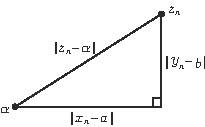
\includegraphics{./Fig/Fig03-A}}
複素数を項とする無限数列 $z_{1}, z_{2}, \ldots, z_{n}, \ldots$ を\textbf{複素数列}とい
う.これを $\{z_{n}\}$ で表す.数列 $\{z_{n}\}$において,$n$ を十分に大きくするとき,$z_n$
が1つの定まった複素数 $\alpha$ に限りなく近づくとき,数列 $\{z_{n}\}$ は$\alpha$に\textbf{収束する}と
いい,これを$\displaystyle \lim_{n\to\infty} z_{n}=\alpha$ あるいは $ z_{n}\to\alpha\, (n\rightarrow\infty)$ のように表す.$z_n$が
$\alpha$に限りなく近づくというのは,点$z_{n}$と$\alpha$の距離
$|z_{n}-\alpha|$ が限りなく0に近づくことである.すなわ
ち $\displaystyle \lim_{n\to \infty}|z_{n}-\alpha|=0$である.$z_{n}=x_{n}+y_{n}i,\, \alpha=a+bi$
とするときは
\[
\begin{array}{lcl}
\dis\lim_{n\rightarrow\infty}z_{n}=\alpha & \Longleftrightarrow &\dis\lim_{n\rightarrow\infty}(x_{n}+y_{n}i)=a+bi\\
&\Longleftrightarrow&\dis \lim_{n\rightarrow\infty}x_{n}=a,\ \lim_{n\rightarrow\infty}y_{n}=b
\end{array}
\]
である.また,数列 $\{z_{n}\}$ が収束しないとき,$\{z_n\}$は\textbf{発散する}という.
\end{Mw}

特に,発散する数列 $\{z_n\}$ について $\displaystyle \lim_{n\rightarrow\infty}|z_{n}|=\infty$ であるとき,$\{z_n\}$は $\infty$ \textbf{に発
散する}といい,$\displaystyle \lim_{n\to\infty} z_{n}=\infty$ あるいは $ z_{n}\rightarrow\infty\, (n\rightarrow\infty)$ と表す.

\noindent
\textbf{[2]\ 無限級数}\par
複素数を項とする無限数列 $\{z_{n}\}$ についても実数列と同様に,「部分和」「無限級数」「無限級数の収束・発散」の意味を定める.
無限級数$\displaystyle \sum^{\infty}_{n=1}z_n$ において,$z_{n}=x_{n}+y_{n}i$ とすると,次が成り立つ.
\[
\sum_{n=1}^{\infty} z_{n}=a+bi\ \Longleftrightarrow\ \sum_{n=1}^{\infty} x_{n}=a,\, \sum_{n=1}^{\infty}y_{n}=b
\]
\step{基本問題を解いてみよう}
\begin{例題}
(1)\ $r >1$ のとき,$\sum_{k=0}^{\infty}\bigg(\displaystyle \frac {\cos x + i \sin x}{r} \bigg)^k
 %%(k= 0,1,2, \ldots)
 $
を求めよ.\par\noindent
(2)\ $\displaystyle r > 1$のとき $\dis \sum_{k=0}^{\infty}\frac{\cos kx}{r^k}$
を求めよ.
\end{例題}

\begin{解答}
(1)  $\dis z = \frac{\cos x + i \sin x}{r}$
とおくと,数列$\{z^k\}\,(k= 0,1,2, \ldots)$の第$n$項までの和$S_n$は
\[
 S_n = 1 + z + z^2 + \cdots + z^{n-1}\quad (n \geqq 1)
\]
$r > 1$であるから$\dis |z| \mathop{=}^{\text{\ajMaruKata{1}}}\footnotetext[1]{$|z|=
\frac{|\cos x+i\,\sin x|}{|r|}=\frac{1}{r}$}
\dfrac{1}{r}<1$\\
したがって\quad$S_n = \frac{1 - z^n}{1 - z}$
\[
\lim_{n \to \infty}\left|S_n - \frac{1}{1-z}\right| \mathop{=}^{\text{\ajMaruKata{2}}} \lim_{n \to \infty}\frac{|z|^n}{|1-z|} = 0
\]よって\footnotetext[2]{$\left|S_n\!-\!\frac{1}{1-z}\right|=
\left|\frac{-z^n}{1-z}\right|=\frac{|z^n|}{|1-z|}=
\frac{|z|^n}{|1-z|}$}
\begin{align*}
\sum_{k=0}^{\infty}z^k &= \lim_{n \to \infty}S_n = \frac{1}{1-z}
=\frac{r}{(r - \cos x) - i \sin x}\\[3mm]
&=\frac{r\{ (r - \cos x) + i \sin x \} }{\{(r - \cos x) - i \sin x\}\{ (r - \cos x) + i \sin x \}}\\[3mm]
&\mathop{=}^{\text{\ajMaruKata{3}}}\frac{r (r - \cos x) + i r \sin x}{r^2 - 2 r \cos x + 1}
\end{align*}\footnotetext[3]{(1行上の分母)$=(r-\cos x)^2+\sin^2x$}
すなわち,求める和は
\[
\sum_{k=0}^{\infty}z^k = \frac{r (r - \cos x)}{r^2 - 2 r \cos x + 1} +i \frac{r \sin x}{r^2 - 2 r \cos x + 1}\tag*{\kotae}
\]

(2)\quad $\begin{array}[t]{lcl}
\dis \sum_{k=0}^{\infty}z^k &=&\dis  \lim_{n \to \infty}\sum_{k=0}^{n}z^k 
\mathop{=}^{\text{\ajMaruKata{4}}} \lim_{n \to \infty}\left( \sum_{k=0}^{n}\frac{\cos kx}{r^k} + i \sum_{k=0}^{n}\frac{\sin kx}{r^k} \right)
\end{array}$\\
であるから,(1)の結果から\footnotetext[4]{ド・モアブルの定理$(\cos x+i\sin x)^k=\cos kx+i\sin kx$}
\[
\sum_{k=0}^{\infty}\frac{\cos kx}{r^k} = \frac{r (r - \cos x)}{r^2 - 2 r \cos x + 1} \tag*{\kotae}
\]

\end{解答}

\section{関数の不定形の極限}
\step{基本を確認しておこう}
一般に,$\lim_{x\to a} f(x)=b,\, \lim_{x\rightarrow a}g(x)=c$であるとき

\begin{Description}{2.5zw}
\item[\hskip1zw a.]
$\lim_{x\rightarrow a} kf (x)=kb$\quad($k$は定数)
\item[\hskip1zw b.]
$\lim_{x\rightarrow a}\{f(x)\pm g(x)\}=b\pm c$\quad(複号同順)
\item[\hskip1zw c.]
$\lim_{x\rightarrow a}f(x)g(x)=bc$
\item[\hskip1zw d.]
$\lim_{x\to a}\dfrac{f(x)}{g(x)}=\dfrac{b}{c}$\quad(ただし,$g(x)\neq 0,\, c\neq 0)$
\end{Description}
が成り立つ.$x\rightarrow a$ の代わりに $x\rightarrow\infty$,$x\rightarrow-\infty$ としても同様に成立する.

しかし,$\lim_{x\to -3}\dfrac{x^{3}+27}{x^{2}-9}, \lim_{x\rightarrow\infty}\dfrac{5x^{2}+4x}{3x^{2}-x+2}, \lim_{x\rightarrow\infty} (\sqrt{x+3}-\sqrt{x})$ などは,形式的には,
$\dfrac{0}{0}$,$\dfrac{\infty}{\infty}$,$\infty-\infty$と表せるが,このままでは実際の極限値は不明である.このよう
な形を\textbf{不定形}と呼ぶが,いろいろな工夫を施して不定形ではないようにする必要
がある.不定形の極限は,上記のほかに $0\times\infty$,$\infty^{0}$,$1^{\infty}$,$0^{0}$ などの形があるが,代表
的なものの処理のコツを次に示す.
\begin{shadebox}
\begin{Description}{8.5zw}
\item[a.\quad $\dfrac{0}{0}$の形]有理式の場合,約分する\\
無理式の場合,分母または分子を有理化する
\item[b.\quad $\dfrac{\infty}{\infty}$の形] 分数式の場合,分母の最高次の項で分母・分子を割る
\item
[c.\quad $\infty-\infty$の形]整式の場合,最高次の項でくくり出す\\
無理式の場合,有理化する\\
$\left(\sqrt{A}-\sqrt{B}=\dfrac{A-B}{\sqrt{A}+\sqrt{B}}\right)$
\end{Description}
\end{shadebox}
\step{基本問題を解いてみよう}
\begin{例題}
次の極限をそれぞれ求めよ.
\begin{longtable}[l]{@{}l@{\hskip1zw}l}
(1)\quad  $\lim_{x\rightarrow 2}\dfrac{\sqrt{x+2}-\sqrt{3x-2}}{\sqrt{4x+1}-\sqrt{5x-1}}$ & (2)\quad $\lim_{x\to -\infty}\dfrac{x^4+3x-8}{2x^3-5x^2+7}$
\\[2mm]
(3)\quad $\lim_{x\rightarrow\infty}(\sqrt{x^{2}-x+1}-\sqrt{x^{2}+3x-1})$&  (4)\quad $\lim_{x\rightarrow\infty}(x-\sqrt{2x+1})$
\end{longtable}
\end{例題}

\begin{解答}\vspace{-\baselineskip}\vspace{-.55\baselineskip}
\begin{fleqn}[4zw]
\begin{alignat}{1}
(1)\ &\phantom{=}\;\lim_{x\to2}\dfrac{\sqrt{x+2}-\sqrt{3x-2}}{\sqrt{4x+1}-\sqrt{5x-1}}\notag\\[3mm]
&=\Mframe{\lim_{x\to2}\dfrac{(x+2-3x+2) (\sqrt{4x+1}+\sqrt{5x-1})}{(4x+1-5x+1)
(\sqrt{x+2}+\sqrt{3x-2})}}\Footnotemark[1]\notag\\[3mm]
&=\lim_{x\to 2}\dfrac{-2(x-2)(\sqrt{4x+1}+\sqrt{5x-1})}{-(x-2)(\sqrt{x+2}+\sqrt{3x-2})}\notag\\[3mm]
&=\lim_{x\rightarrow 2}\dfrac{2(\sqrt{4x+1}+\sqrt{5x-1})}{\sqrt{x+2}+\sqrt{3x-2}}=\dfrac{2(3+3)}{2+2}=3\tag*{\hbox to1zw{\hss\Kotae}}
\end{alignat}\footnotetext[1]{分母・分子がともに無理式で,$\frac{0}{0}$の不定形の場合,分母・分子の両方を有理化する.}
\end{fleqn}

\noindent
(2)\quad$\Mframe{x=-t}\Footnote[2]{$\lim_{x\to-\infty}f(x)$は$x=-t$とおいて,
$\lim_{t\to\infty}g(t)$の形に帰着させる.}$とおくと,$x\to-\infty$のとき$t\to\infty$.
\begin{align*}
&\lim_{x\rightarrow-\infty}\dfrac{x^{4}+3x-8}{2x^{3}-5x^{2}+7}\\
=\;&\Mframe{\lim_{t\rightarrow\infty}\dfrac{t^{4}-3t-8}{-2t^{3}-5t^{2}+7}}\Footnotemark[3]
=\lim_{t\rightarrow\infty}\dfrac{t-\dfrac{3}{t^{2}}-\dfrac{8}{t^{3}}}{-2-\dfrac{5}{t}+\dfrac{7}{t^{3}}}=-\infty\tag*{\Kotae}
\end{align*}%
\footnotetext[3]{$\frac{\infty}{\infty}$の不定形
である.分母の最高次の項で分母・分子を割る.}\footnotetext[4]{無理式で$\infty-\infty$の不定形である.与式
$=\frac{\sqrt{\quad}\;\text{\raisebox{-.5mm}{$-$}}\;\sqrt{\quad}}{1}$と考えて,分子を有理化する.}
\begin{fleqn}
\begin{alignat*}{2}
(3)\quad&\dis\Mframe{\lim_{x\to\infty}(\sqrt{x^{2}-x+1}-\sqrt{x^{2}+3x-1})}\Footnotemark[4]\\[3mm]
&\dis=\lim_{x\rightarrow\infty}\dfrac{(x^{2}-x+1)-(x^{2}+3x-1)}{\sqrt{x^{2}-x+1}+\sqrt{x^{2}+3x-1}}\\[3mm]
&\dis=\lim_{x\rightarrow\infty}\dfrac{-4x+2}{\sqrt{x^{2}-x+1}+\sqrt{x^{2}+3x-1}}\\[3mm]
&\dis\mathop{=}^{\text{\ajMaruKata{5}}}\lim_{x\rightarrow\infty}\dfrac{-4+\dfrac{2}{x}}{\sqrt{1-\dfrac{1}{x}+\dfrac{1}{x^{2}}}+\sqrt{1+\dfrac{3}{x}-\dfrac{1}{x^{2}}}}
=\dfrac{-4}{2}=-2\tag*{\Kotae}
\end{alignat*}
\footnotetext[5]{分母・分子を$\sqrt{x^2}=x$で割った.}

\footnotetext[6]{$\infty-\infty$の不定形で無理式だから有理化をしそうであるが,$x$と$\sqrt{2x+1}$では$x$のほうが高次だから$x$でくくった.}
\begin{alignat*}{2}
(4)\quad&\lim_{x\rightarrow\infty}(x-\sqrt{2x+1})\\
&\mathop{=}^{\text{\ajMaruKata{6}}} \lim_{x\rightarrow\infty}x\left(1-\dfrac{\sqrt{2x+1}}{x}\right)
=\lim_{x\rightarrow\infty}x\left(1-\sqrt{\dfrac{2}{x}+\dfrac{1}{x^2}}\right)
\mathop{=}^{\text{\ajMaruKata{7}}}\infty\tag*{\Kotae}
\end{alignat*}\footnotetext[7]{$\infty\times1$より極限は$\infty$.}
\end{fleqn}
\end{解答}


\section{重要な極限(1)}
\step{基本を確認しておこう}

三角関数についての$ \frac{0}{0}$ の不定形である.

三角関数の不定形の極限では,次の2つの公式に帰着させて考えるのが原則である.

\begin{shadebox}
\begin{center}
\mbox{$\lim_{\Textcircled{$\theta$} \rightarrow 0}\frac{\sin \Textcircled{$\theta$}}{\Textcircled{$\theta$}} =1,\quad \lim_{\theta \rightarrow 0}\frac{\tan\theta}{\theta}=1 \quad \mbox{\small(ただし,$\theta$は弧度法で表されている)}$}
\end{center}
\end{shadebox}

たとえば,$ab\neq 0$ のとき $\lim_{\theta \rightarrow 0}\frac{\sin a\theta}{b\theta}=\lim_{\theta\rightarrow 0}\frac{\sin a\theta}{a\theta}\cdot\frac{a}{b}=1\cdot\frac{a}{b}=\frac{a}{b}$
\begin{align*}
\lim_{\theta\rightarrow 0}\frac{1-\cos\theta}{\theta^{2}}&=\lim_{\theta\rightarrow 0}\frac{(1-\cos\theta)(1+\cos\theta)}{\theta^{2}(1+\cos\theta)}=\lim_{\theta\rightarrow 0}\frac{\sin^{2}\theta}{\theta^{2}(1+\cos\theta)}\\
&=\lim_{\theta\rightarrow 0}\left(\frac{\sin\theta}{\theta}\right)^{2}\cdot\frac{1}{1+\cos\theta}=1^{2}\cdot\frac{1}{2}=\frac{1}{2}
\end{align*}
となる.この2つの結果は公式として覚えておくとよい.

さらに,$a\neq 0$ のとき
\[
\lim_{x \rightarrow \infty}x\sin\frac{a}{x}=\lim_{t \rightarrow 0}\frac{\sin at}{t}=a \quad \left(x=\frac{1}{t} とおいた \right)
\]
となる.ただし,$\lim_{x\rightarrow 0}x\sin\frac{1}{x}$ は $\left |\sin\frac{1}{x}\right |\leqq 1$ から $0\leqq \left |x\sin\frac{1}{x}\right |\leqq |x|$ となり,はさみうちの原理から与式 $=0$ となる.

\step{基本問題を解いてみよう}
\begin{例題}
次の極限を求めよ.\par
\begin{longtable}[l]{@{}l@{\hskip4zw}l}
(1)\quad$\lim_{x\rightarrow 0}\frac{\cos 7x-\cos 3x}{x^{2}}$ & (2)\quad$\lim_{x\rightarrow 0}\frac{\tan^{3}x-\sin^{3}x}{x^{5}}$\\[3mm]
(3)\quad$\lim_{x\rightarrow \frac{\pi}{2}}\frac{1-\cos(1-\sin x)}{\cos^{4}x}$&
\end{longtable}
\end{例題}

\begin{解答}
\begin{fleqn}[4zw]
$\begin{array}[t]{ll}
(1)\quad\cos 7x-\cos 3x\, &\mathop{=}^{\text{\ajMaruKata{1}}}-2\sin\frac{7x+3x}{2}\sin\frac{7x-3x}{2}\\[3mm]
&=-2\sin 5x\sin 2x \quad から
\end{array}$\footnotetext[1]{和積の公式
$\cos A-\cos B=-2\sin\frac{A+B}{2}\sin\frac{A-B}{2}$より.
}\par
\begin{alignat}{2}
&与式\, &=&\lim_{x\rightarrow 0}\frac{-2\sin 5x\sin 2x}{x^{2}}=\lim_{x\rightarrow 0}(-2)\cdot\frac{\sin 5x}{5x}\cdot \frac{\sin 2x}{2x}\cdot 10\notag\\[3mm]
&&=&\;(-2)\cdot 1\cdot 1\cdot 10=-20\tag*{\kotae}
\end{alignat}
\end{fleqn}
\begin{fleqn}[1.5zw]
$(2)\quad\lim_{x\rightarrow 0}\frac{\tan^{3}x-\sin^{3}x}{x^{5}}=\lim_{x\rightarrow 0}\frac{\sin^{3}x(1-\cos^{3}x)}{x^{5}\cos^{3}x}$\\
\begin{alignat}{2}
&&=&\lim_{x \rightarrow 0}\frac{\sin^3 x(1-\cos x)(1+\cos x+\cos^{2}x)}{x^{5}\cos^{3}x}\notag\\[3mm]
&&\mathop{=}^{\text{\ajMaruKata{2}}}&\lim_{x \rightarrow 0}\frac{\sin^3x\sin^2x(1+\cos x+\cos^{2}x)}{x^{5}(1+\cos x)\cos^{3}x}\notag\\[3mm]
&&=&\lim_{x\rightarrow 0}\left (\frac{\sin x}{x}\right )^{5}\cdot\frac{1+\cos x+\cos^{2}x}{(1+\cos x)\cos^{3}x}=1\cdot\frac{3}{2\cdot 1}=\frac{3}{2}\tag*{\Kotae}
\end{alignat}\footnotetext[2]{分母・分子に$1+\cos x$を掛けた.あるいは
$1-\cos x=2\sin^2\frac{x}{2}$を用いてもよい.}
$(3)\quad\frac{\pi}{2}-x=t とおくと \cos x=\cos\left (\frac{\pi}{2}-t\right )=\sin t\\
\quad1-\sin x=1-\sin\left (\frac{\pi}{2}-t\right )=1-\cos t\mathop{=}^{\text{\ajMaruKata{3}}}2\sin^{2}\frac{t}{2}$\footnotetext[3]{半角の公式より.}\footnotetext[4]{%
	分子に再び半角の公式を用いた.
	}\footnotetext[5]{$t\to0$のとき$\sin^2\frac{t}{2}\to0$より,
	$\sin^2\frac{t}{2}=\theta$とすると
	$\lim_{t\to0}\frac{\sin\left(\sin^2\frac{t}{2}\right)}{\sin^2\frac{t}{2}}
	=\lim_{\theta\to0}\frac{\sin\theta}{\theta}=1
	$となる.}
\begin{alignat}{2}
&与式\, &=&
\lim_{t\rightarrow 0}\frac{1-\cos\left (2\sin^{2}\frac{t}{2}\right )}{\sin^{4}t}\notag\mathop{=}^{\text{\ajMaruKata{4}}}\lim_{t\rightarrow 0}\frac{2\sin^{2}\left (\sin^{2}\frac{t}{2}\right )}{\sin^{4}t}\notag\\[3mm]
&&=&\lim_{t\rightarrow 0}2\left (\frac{t}{\sin t}\right )^{4}\cdot
\Mframe{\left\{\frac{\sin\left (\sin^{2}\frac{t}{2}\right )}{\sin^{2}\frac{t}{2}}\right\}^{2}}\Footnotemark[5]\cdot\left (\frac{\sin\frac{t}{2}}{\frac{t}{2}}\right )^{4}\cdot\frac{1}{2^{4}}\notag\\[3mm]
&&=&\;2\cdot 1\cdot 1\cdot 1\cdot\frac{1}{2^{4}}=\frac{1}{8}\tag*{\kotae}
\end{alignat}
\end{fleqn}
\end{解答}

\section{重要な極限(2)}
\step{基本を確認しておこう}

次の定義はきわめて重要である.

\begin{shadebox}
\begin{center}
$\lim_{\text{\Textcircled{$h$}} \rightarrow 0}(1+\Textcircled{$h$})
^{\frac{1}{\text{\Textcircled{$h$}}}} = e \quad (e=2.71828 \cdots)$
\end{center}
\end{shadebox}

\VS{-.5}
$e$は\textbf{自然対数の底}と呼ばれる無理数である.これより次の公式が導かれる.

\begin{titlebox}{指数関数・対数関数に関する極限}
\begin{fleqn}
\begin{align*}
(1)\ &\lim_{x \rightarrow \pm \infty}\left(1+\frac{1}{x}\right)^x = e\hskip4zw
(2)\ \lim_{x \rightarrow 0}\frac{e^x - 1}{x} = 1\\
(3)\ &\lim_{x \rightarrow 0}\frac{a^x - b^x}{x} = \log_e\frac{a}{b} \enskip(a>0,\,b>0)
\end{align*}
\end{fleqn}
\end{titlebox}
\begin{証明}(1)\ 
$x = \frac{1}{h}$ とおくと,$
\lim_{x\rightarrow\pm\infty}\left(1+\frac{1}{x}\right)^{x}=\lim_{h\rightarrow\pm 0}(1+h)^{\frac{1}{h}}=e$
\\
(2)\ $e^{x}-1=h$ とおくと $x=\log_{e}(1+h)$ で $h\rightarrow 0$ だから
\[
\lim_{x\rightarrow 0}\frac{e^{x}-1}{x}=\lim_{h\rightarrow 0}\frac{h}{\log_{e}(1+h)}=\lim_{h\rightarrow 0}\frac{1}{\log_{e}(1+h)^{\frac{1}{h}}}=\frac{1}{\log_{e}e}=1
\]
(3)\ $a>0,\, b>0$ のとき
\begin{align*}
\lim_{x\rightarrow 0}\frac{a^{x}-b^{x}}{x}&=\lim_{x\rightarrow 0}\frac{b^{x}\{(\frac{a}{b})^{x}-1\}}{x}=\lim_{x\rightarrow 0}b^{x}\cdot\lim_{x\to0}\frac{(\frac{a}{b})^{x}-1}{x}\\
&=1\cdot\log_{e}\frac{a}{b}=\log_{e}\frac{a}{b}
\end{align*}
\begin{shadebox}
$a>1$のとき,$\lim_{x\to \infty}\frac{x}{a^x}=0$
\end{shadebox}
\end{証明}

\begin{証明}
$x\to\infty$より,十分大きな自然数$n$に対して$n\le x<n+1$として考えると,$a^x\ge a^n\,(>0)$だから
\[
0<\frac{x}{a^x}<\frac{n+1}{a^n}
\]
$a>1$のとき$a=1+h\,(h>0)$とおけるから,2項定理により$n\ge2$のとき
\begin{align*}
a^n & = (1+h)^n= {}_n\mathrm{C}_0+{}_n\mathrm{C}_1\,h+{}_n\mathrm{C}_2\,h^2+\cdots+{}_n\mathrm{C}_n\,h^n\\
&>{}_n\mathrm{C}_2\,h^2=\frac{n(n-1)}{2}h^2\,(>0)
\intertext{ゆえに}
&\frac{n+1}{a^n}<\frac{n+1}{\frac{n(n-1)}{2}h^2}=
\frac{2(n+1)}{n(n-1)h^2}=\frac{2(1+\frac{1}{n})}{(n-1)h^2}
\end{align*}
ここに,$x\to \infty$のとき$n\to\infty$であるから,
\[
0\le\lim_{x\to\infty}\frac{x}{a^x}\le\lim_{n\to\infty}\frac{n+1}{a^n}
\le\lim_{n\to \infty}\frac{(1+\frac{1}{n})}{(n-1)h^2}=0
\]
よって,はさみうちの原理から
\[
a>1のとき\quad \lim_{x\to\infty}\frac{x}{a^x}=0\tag*{(証明終)}
\]
\end{証明}
\step{基本問題を解いてみよう}
\begin{例題}
次の極限を求めよ.

\begin{fleqn}
\begin{alignat*}{2}
(1)\quad & \lim_{x\rightarrow 0}\frac{\log_{2}(a+3x)-\log_{2}a}{x}\quad && (a>0)\\
(2)\quad& \lim_{x\rightarrow 0}\frac{e^{\sin 3x}-e^{-2x}}{x} && (3)\enskip\lim_{x\rightarrow\infty}\left(1+\frac{1}{x}+\frac{1}{x^2}\right)^2
\end{alignat*}
\end{fleqn}
\end{例題}

\enlargethispage{3mm}
\begin{解答}\vspace{-1.5\baselineskip}
\begin{align*}
(1)\enskip&\lim_{x \rightarrow 0}\frac{\log_2(a + 3x) - \log_2a}{x}\\
&=\lim_{x \rightarrow 0}\frac{\log_2\left(1 + \frac{3x}{a}\right)}{x} 
\mathop{=}^{\text{\ajMaruKata{1}}} \lim_{x \rightarrow 0}\frac{\log_2\left(1 + \frac{3x}{a}\right)}{\frac{3x}{a}} \cdot \frac{3}{a}\\
&=\lim_{x \rightarrow 0}\frac{3}{a}\log_2\left(1 + \frac{3x}{a}\right)
^{\frac{1}{\frac{3x}{a}}} = \frac{3}{a}\log_2e\tag*{\kotae}
\end{align*}\footnotetext[1]{%
	$\lim_{f(x)\to0}\{1+f(x)\}^{\frac{1}{f(x)}}=e$を用いるために,
	分母を$\frac{3x}{a}$に直した.
	}
\begin{fleqn}
\begin{align*}
(2)\enskip&\lim_{x \rightarrow 0}\frac{e^{\sin3x}-e^{-2x}}{x}\mathop{=}^{\text{\ajMaruKata{2}}}\lim_{x \rightarrow 0}\frac{e^{\sin3x}-1-(e^{-2x}-1)}{x}\\
&=\lim_{x \rightarrow 0}\left(\frac{e^{\sin3x}-1}{\sin3x}\cdot \frac{\sin3x}{3x}\cdot 3 + \frac{e^{-2x}-1}{-2x}\cdot2\right)\\
&=1\cdot 1\cdot 3+1\cdot 2=5\tag*{\kotae}
\end{align*}\footnotetext[2]{%
	$\lim_{f(x)\to0}\frac{e^{f(x)}-1}{f(x)}=1$を用いるために,分子を変形した.
	}%
\end{fleqn}%
%(3)\quad \Mframe{xは十分大きい正の数と考えてよい}\Footnote[3]{%
%	$x\to\infty$より.
%	}ので,自然数 $n$ に対して $n\leqq x<n+1$ とすると
%\[
%\Mframe{\dis
%0<\frac{x}{3^{x}}<\frac{n+1}{3^{n}}}
%\Footnotemark[4]\tag*{$\cdots\cdots$ ①}
%\]
%
%ここで,\Mframe{2項定理}\footnotetext[4]{$y=3^x$のグラフは単調増加だから,$n<2^n\leq3^x<3^{n+1}$より
%$\frac{1}{3^{n+1}}<\frac{1}{3^x}\leq\frac{1}{3^n}$
%したがって$0<\frac{n}{3^{n+1}}<\frac{x}{3^x}<\frac{n+1}{3^n}$
%}\Footnote[5]{%
%	$(a+b)^n={}_n\mathrm{C}_0a^n+{}_n\mathrm{C}_1a^{n-1}b
%	+\cdots+{}_n\mathrm{C}_r a^{n-r}b^r
%	+\cdots+{}_n\mathrm{C}_nb^n
%	$
%	}により $n\geqq 2$ のとき
%\begin{align}
%3^{n}&=(1+2)^{n}={}_n\mathrm{C}_0 + {}_n\mathrm{C}_1 \cdot 2+{}_n\mathrm{C}_2 \cdot 2^2 + \cdots + {}_n\mathrm{C}_n2^n\notag\\
%&>{}_n\mathrm{C}_2\cdot 2^2=\frac{n(n-1)}{2}\cdot 2^{2}=2n(n-1)\tag*{$\cdots\cdots$②}
%\end{align}
%
%①, ②から\par
%\[
%0<\frac{x}{3^{x}}<\frac{n+1}{2n(n{-1)}}=\frac{1+\frac{1}{n}}{2(n-1)}
%\]
%ここに,$ x\rightarrow\infty$ のとき $ n\rightarrow\infty$ だから\par
%\[
%0\leqq \lim_{x \rightarrow \infty}\frac{x}{3^{x}}\leqq \lim_{x \rightarrow \infty}\frac{1+\frac{1}{n}}{2(n{-1)}}=0
%\]
%
%よって,はさみうちの原理から
%\[
%\lim_{x \rightarrow \infty}\frac{x}{3^{x}}=0 \tag*{\kotae}
%\] 
\end{解答}%%
(3)$\displaystyle \lim_{x \to \infty} \left( 1+\frac{1}{x}+\frac{1}{x^2} \right)^x$ において,
$x=\dfrac{1}{y}$とおくと$x \to \infty$のとき$y \to 0$\\
したがって,
\[
 \lim_{x \to \infty} \left( 1+\dfrac{1}{x}+\dfrac{1}{x^2} \right)^x
=\lim_{y \to 0} (1+y+y^2)^{\frac{1}{y}}
\]
さらに
$\Mframe{y+y^2=z\text{とおく}}\Footnote[3]{$y \to 0$のとき$y+y^2 \to 0 $であるから,
$\displaystyle \lim_{z \to 0} (1+z)^\frac{1}{z} =1$を用いることができるのではないかと予想して$y+y^2=z $とおいた.}$
と,$y \to 0$のとき$z \to 0$であり
\[
 \lim_{y \to 0} (1+y+y^2)^{\frac{1}{y}}
=\lim_{\begin{subarray}{c}
	y \to 0\\ z \to 0
	\end{subarray}
	}    (1+z)^{\frac{1}{y}}
=\lim_{
	\begin{subarray}{c}
	y \to 0\\
	z \to 0
	\end{subarray}
	} \{ (1+z)^{\frac{1}{z}} \}^{\frac{z}{y}}
\]
ここで,
$\displaystyle 
 \lim_{y \to 0} \frac{z}{y}  
=\lim_{y \to 0} \frac{y+y^2}{y} =\lim_{y \to 0} (1+y) =1$

よって,$\text{与式}=e^1=e  $\kotae
\pagebreak[3]

\section{微分係数の定義}
\step{基本を確認しておこう}

\begin{Mw}{45mm}{\hfill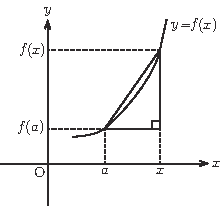
\includegraphics{./Fig/Fig03-B}}
連続関数 \mbox{$y=f(x)$}の定義域内の2点 $a,\linebreak x$ に対して $\lim_{x\rightarrow a}\frac{f(x)-f(a)}{x-a}$,すなわち,$\lim_{h\rightarrow 0}\frac{f(a+h)-f(a)}{h}$ が存在して有限確定ならば,$x=a$ において\textbf{微分可能}といい,この極限値を関数 $f(x)$ の $x=a$ における\textbf{微分係数}あるいは,\textbf{微係数}といい,$f'(a)$ と表す.また,
\begin{align*}
&\lim_{x\rightarrow a+0}\frac{f(x)-f(a)}{x-a}\quad すなわち \quad \lim_{h\rightarrow+0}\frac{f(a+h)-f(a)}{h}\\
&\lim_{x\rightarrow a-0}\frac{f(x)-f(a)}{x-a}\quad すなわち \quad \lim_{h\rightarrow-0}\frac{f(a+h)-f(a)}{h}
\end{align*}
が存在して有限確定ならば,それぞれ $x=a$ において\textbf{右側微分可能},\textbf{左側微分可能}といい,これらの極限値を $f_{+}'(a)$,$f_{-}'(a)$ と表し,関数 $f(x)$ の $x=a$ における\textbf{右側微分係数},\textbf{左側微分係数}という.
\end{Mw}

\begin{shadebox}
\centering
$f(x)$が$x=a$で微分可能\quad$\Longleftrightarrow$\quad$f_{+}'(a)=f_{-}'(a)$
\end{shadebox}
\pagebreak[3]

\VS{-.5}
さて,微分可能な関数 $f(x)$ は連続である.

\begin{証明}$f(x)$ が $x=a$ で微分可能であるならば,
\[
\lim_{x\rightarrow a}\{f(x)-f(a)\}=\lim_{x\rightarrow a}\frac{f(x)-f(a)}{x-a}\cdot(x-a)=f'(a)\cdot 0=0
\]
よって,$\lim_{x\rightarrow a}f(x)=f(a)$ となり,$f(x)$ は $x=a$ で連続である.\hfill(証明終)
\end{証明}

\step{基本問題を解いてみよう}
\begin{例題}
次の関数の与えられた点における微分係数を定義により求めよ.\par
\begin{longtable}[l]{@{}ll}
(1)\quad$f(x)=\frac{1}{x}\quad (x=a\neq 0)$ &(2)\quad$f(x)=\sqrt[3]{x}\quad (x=a)$ \\[3mm]
(3)\quad$f(x)=\left\{\begin{array}{ll}
x\sin\frac{1}{x} & (x\neq 0)\\
0 & (x=0)
\end{array}\right.$
\quad$(x=0)$
\end{longtable}
\end{例題}

\begin{解答}$(1)\quad f'(a) = \lim_{h \rightarrow 0}\frac{f(a+h)-f(a)}{h}$
\[
=\lim_{h \rightarrow 0}\frac{1}{h}\left (\frac{1}{a+h} - \frac{1}{a} \right) =\lim_{h \rightarrow 0}\frac{-1}{(a+h)a}=-\frac{1}{a^2}\tag*{\kotae}
\]
\begin{別解}
$f'(a)=\lim_{x\to a}\frac{f(x)-f(a)}{x-a}=\lim_{x\to a}
\frac{\frac{1}{x}-\frac{1}{a}}{x-a}$
\end{別解}
\begin{fleqn}[1.5zw]
(2)\hspace{1zw}(i)\quad $a \neq 0$のとき
\begin{alignat}{2}
&f'(a) &=&\lim_{x\rightarrow a}\frac{f(x) - f(a)}{x-a}=\lim_{x\rightarrow a}\frac{\sqrt[3]{x} - \sqrt[3]{a}}{x-a}\notag\\[3mm]
&&=&\lim_{x\rightarrow a}\frac{\sqrt[3]{x} - \sqrt[3]{a}}{(\sqrt[3]{x} - \sqrt[3]{a})(\sqrt[3]{x^2} + \sqrt[3]{x}\sqrt[3]{a} + \sqrt[3]{a^2})}\notag\\[3mm]
&&=&\lim_{x\rightarrow a}\frac{1}{\sqrt[3]{x^2} + \sqrt[3]{x}\sqrt[3]{a} + \sqrt[3]{a^2}} \mathop{=}^{\text{\ajMaruKata{1}}}\frac{1}{3\sqrt[3]{a^2}}\tag*{\kotae}
\end{alignat}\footnotetext[1]{最初から$a\not=0$と$a=0$の場合分けには気づかないかもしれないが,\ajMaruKata{1}の所で場合分けに気づくことになる.}%
(ii)\quad$a = 0$のとき
\[
f'(0) =\lim_{x\rightarrow 0}\frac{f(x) - f(0)}{x}=\lim_{x\rightarrow0}\frac{\sqrt[3]{x}}{x} = \lim_{x\rightarrow 0}\frac{1}{\sqrt[3]{x^2}}
=\infty\tag*{\kotae}
\]
(3)\hspace{1zw}$\lim_{x\rightarrow 0}\frac{f(x) - f(0)}{x}=\lim_{x\rightarrow 0}\frac{x \sin \frac{1}{x}}{x}=\lim_{x\rightarrow 0}\sin \frac{1}{x}$
%
%\Mframe{\sin\frac{1}{x}はx \rightarrow 0のとき有限確定値あるいは\infty,-\infty のいずれにもならない}\,\Footnote[2]{%
%	$x=\frac{1}{\pi},\frac{1}{2\pi},\ldots,\frac{1}{n\pi},\ldots$の値をとりながら,$x\to0$のとき$\lim_{x\to0}\sin\frac{1}{x}=0x=\frac{2}{\pi},\frac{2}{5\pi},\ldots,\frac{2}{(4n+1)\pi},\ldots$の値をとりながら,$x\to0$のとき$\lim_{x\to0}\sin\frac{1}{x}=1$両者が一致しないので,極限は存在しない.
%	}\linebreak
%	ので,$f'(0)$は存在しない.\kotae

$x>0$において,$\sin \dfrac{1}{x}=0$となるのは
$\dfrac{1}{x}=n\pi$より$x=\dfrac{1}{n\pi}\, (n=1,2,\ldots)$のときである.

また,$\sin \dfrac{1}{x}=1$となるのは
$\dfrac{1}{x}=\dfrac{\pi}{2}+2(n-1)\pi=\dfrac{4n-3}{2}\pi$より
$x=\dfrac{1}{(4n-3)\pi}\, (n=1,2,\ldots)$のときである.

したがって,$x=\dfrac{1}{\pi},\, \dfrac{1}{2\pi},\, \ldots , \, \dfrac{1}{n\pi}, \ldots$の値をとりながら
$x$が限りなく0に近づくとき,$\sin \dfrac{1}{x}$の値はつねに0となる.

また,$x=\dfrac{2}{\pi}, \, \dfrac{2}{5\pi}, \, \ldots , \,  \dfrac{1}{(4n-3)\pi}, \, \ldots$の値をとりながら
$x$が限りなく0に近づくとき,$\sin \dfrac{1}{x}$の値はつねに1となる.

これらの結果から$\displaystyle \lim_{x \to 0} \sin \frac{1}{x}$は存在しない.

よって,$f'(0)$は存在しない.\kotae

\end{fleqn}

\step{過去問題にチャレンジ!}
\medskip
\begin{問題}[1]
正の整数$n$ に対して,$1\times 3\times \cdots \times( 2n-1 )=( 2n-1 )!!$ と表すことにします.
このとき,次の極限値を求めなさい.
\[
\lim_{n\to\infty}\frac{\sqrt[n]{( 2n-1)!!}}{n}
\]
\end{問題}
\begin{解答}
自然対数をとって考える.$(2n-1)!!=\frac{(2n)!}{(2n)!!}$より
\begin{fleqn}
\begin{align*}
&\log_{e}\frac{\sqrt[n]{\left( 2n-1 \right)!!}}{n}=\log_{e}\frac{1}{n}\sqrt[\text{\raisebox{3mm}{\scalebox{1.1}{$n$}}}]{\frac{(2n)!}{(2n)!!}}\\
	=&\;\log_{e}\sqrt[\text{\raisebox{3mm}{$n$}}]{\left(\frac{n}{2}\times \frac{n}{4}\times\cdots\times
\frac{n}{2n} \right)\times \left(\frac{1}{n}\times \frac{2}{n}\times\cdots\times \frac{2n}{n} \right)}\\
	=&\;
\frac{1}{n}\left(\sum\limits_{k=1}^n \log_{e}
\frac{n}{2k}+\sum_{k=1}^{2n} \log_{e}
\frac{k}{n}\right)
=\frac{1}{n}\sum\limits_{k=1}^n \left\{-\log_{e}\left(
2\cdot \frac{k}{n}\right) \right\} +\frac{1}{n}\sum\limits_{k=1}^{2n} \log_{e}\frac{k}{n} 
\end{align*}
\end{fleqn}
 よって
\begin{fleqn}[2zw]
\begin{align*}
&\lim_{n\to\infty}\log_{e}\frac{\sqrt[n]{\left(2n-1\right)!!}}{n}\\
&=\lim_{n\to\infty}\frac{1}{n}\sum\limits_{k=1}^n
\left\{-\log_{e}\left(2\cdot \frac{k}{n} \right) \right\}+\lim_{n\to\infty}
\frac{1}{n}\sum\limits_{k=1}^{2n} \log_{e}\frac{k}{n}\\
&=-\int_{0}^1 \log_{e} 2x\, dx+\int_0^2\log_{e}x\,dx\\
&=-[x\log_e2x-x]_0^1+[x\log_e x-x]_0^2=\log_e\frac{2}{e}
\end{align*}
\end{fleqn}
ゆえに
\[
\lim_{n\to\infty}
\frac{\sqrt[n]{(2n-1)!!}}{n}=\frac{2}{e}\tag*{\Kotae}
\]
\end{解答}
\begin{解説}
\Mframe{区分求積法}\Footnote[1]{第3章9節で学ぶ.}を用いる.なお次も有用である.
\end{解説}
\begin{titlebox}{スターリングの公式}
$n\to \infty$のとき(両辺の比$\to1$という意味で)
\[
n!\sim \sqrt{2\pi n}\left(\frac{n}{e} \right)^{n}\hskip3zw
\text{\null($e$は自然対数の底)}
\]
\end{titlebox}
これを用いると,$n\to \infty $のとき,次のようにも求められる.
\begin{fleqn}
\begin{align*}
\frac{\sqrt[\text{\raisebox{1.5mm}{$n$}}]{\left( 2n-1 \right)!!}}{n}
 &=\frac{1}{n}\sqrt[\text{\raisebox{3mm}{$n$}}]{\frac{(2n)!}{2^{n}\times n!}}\, \sim \, 
\frac{1}{2n}\sqrt[\text{\raisebox{3mm}{$n$}}]{\sqrt {2\pi \times 2n} \left( \frac{2n}{e} 
\right)^{2n}\div \sqrt {2\pi n} \left( \frac{n}{e} \right)^{n}}\\
& =\frac{1}{2n}\sqrt[\text{\raisebox{2.8mm}{$n$}}]{\sqrt{2}\! \times\! 2^{2n}\!\times\! 
\left(\frac{n}{e} \right)^{n}}\!\! =\frac{1}{2n}\times \frac{n}{e}\times 
4\times\!\! \sqrt[2n]{2}= \frac{2}{e}\times\!\! \sqrt[{2n}]{2}\sim \frac{2}{e}
\end{align*}
\end{fleqn}
\begin{問題}[2]
$f(x)$は\Mframe{C^{n}級}\Footnote[2]{第2章で学ぶ.}の関数($f'(x),f''(x),\ldots,f^{(n)}(x):\,n$次までの導関数が連続な関数)とし,しかも$f(0)=f'(0)=\cdots =f^{(n)}(0)=0$と仮定します.

$
\lim_{x\to0}\frac{f^{(n)}(x)\cdot \sin x}{f^{(n-1)}(x)}=1$ 
のとき,$\lim_{x\to0}\frac{f^{(n)}(x)}{f(x)}(\sin x)^{n}$を求めなさい.
\end{問題}


\begin{解答}
\begin{fleqn}[2zw]
\[
\frac{f^{(n)}(x)}{f(x)}(\sin x)^{n}=\frac{f^{(n)}(x)\sin x}{f^{( n-1 )}( x )}\times\frac{f^{( n-1 )}( x )\sin x}{f^{( n-2 )}( x )}\times \cdots \times \frac{f^{(1)}(x)\sin x}{f( x )}
\]
\end{fleqn}
\end{解答}
ロピタルの定理より
\begin{fleqn}[4zw]
\begin{align*}
\lim_{x\to0}\frac{f^{(n-1)}(x)\sin x}{f^{(n-2)}(x)}&=\lim_{x\to0} \frac{\{f^{(n-1)}(x)\cdot \sin x \}'}{\{f^{(n-2)}(x) \}'}\\
	& =\lim_{x\to0} \frac{f^{(n)}(x)\sin x +f^{(n-1)}(x)\cos x}{f^{(n-1)}(x)}\\
	&=1+\lim_{x\to0}\cos x=2\\
\lim_{x\to0}\frac{f^{(n-2)}(x)\sin x}{f^{(n-3)}(x)}
	&=\lim_{x\to0}\frac{\{f^{(n-2)}(x)\sin x \}'}{\{ f^{(n-3)}(x)\}'}\\
	&=\lim_{x\to0}\frac{f^{(n-1)}(x)\sin x+f^{(n-2)}(x)\cos x}{f^{(n-2)}(x)}\\
	&=2+\lim_{x\to0}\cos x=3\\
	&\vdots\\
\lim_{x\to0}\frac{f^{(n-k+1)}(x)\sin x}{f^{(n-k)}(x)}
	&=k\quad\text{($k$は実数,$1\leq  k\leq  n$)}
\end{align*}
\end{fleqn}
よって,
\begin{fleqn}[4zw]
\begin{align*}
&\lim_{x\to0}\frac{f^{(n)}(x)}{f(x)}(\sin x)^{n}\\
=&\;\lim_{x\to0}
	\left\{\frac{f^{(n)}(x)\sin x}{f^{(n-1)}(x)}\!\times\!
		\frac{f^{(n-1)}(x)\sin x}{f^{(n-2)}(x)}
		\!\times\!\cdots\!\times\!
			\frac{f^{(1)}(x)\sin x}{f(x)}\right\}\\
			=&\;1\cdot 2\cdot\, \cdots\, \cdot n=n!\tag*{\Kotae}
\end{align*}
\end{fleqn}
\end{解答}
\begin{解説}
 次の定理を用いて不定形の極限を求める.

\begin{titlebox}{ロピタルの定理}
\begin{fleqn}[4zw]
$f(x),g(x)$が$x=a$を含む区間で連続かつ$x=a$ 以外で微分可能で
\[
\lim_{x\to a}f(x)=\lim_{x\to a}g(x)=0
\]
とするとき
\[
\lim_{x\to a}\frac{f'(x)}{g'(x)}\text{が存在するならば}
\lim_{x\to a}\frac{f(x)}{g(x)}=\lim_{x\to a}\frac{f'(x)}{g'(x)}
\]
\end{fleqn}
\end{titlebox}
\end{解説}

